\Appendix{Post processing of particle data}
\label{app:project-SPH-grid}    

\begin{figure}[!htb]
    \centering
	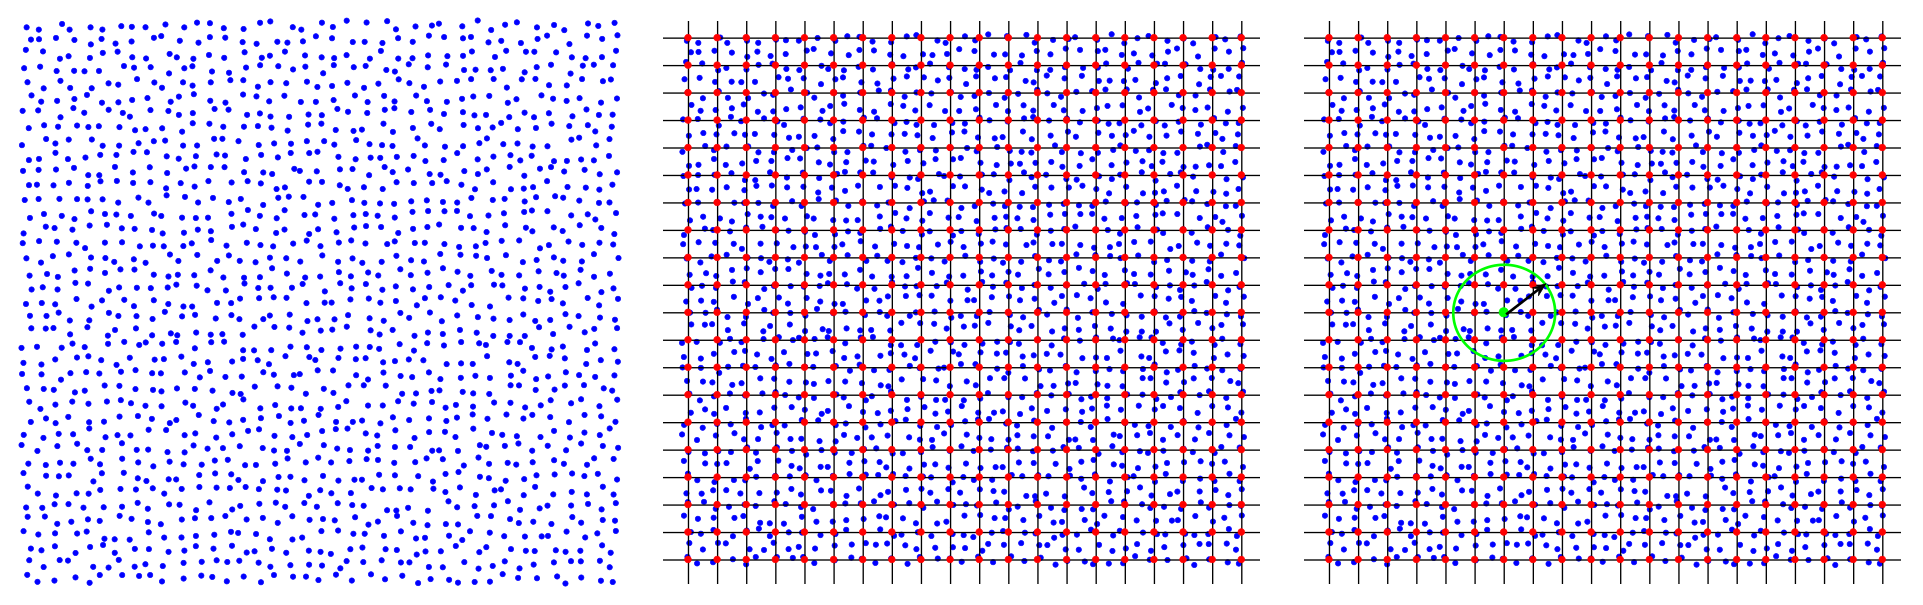
\includegraphics[width=14cm]{Appendix-D/Figures/FigA1.png} 
    \caption{Procedure of projection of simulation results carried by particles onto regular grids. Figures from left to right are: 1) raw data of SPH simulation results (irregularly distributed in space), 2) Add regular mesh, 3) searching for neighbours of each node (the blue SPH particles within the green circle around the red dot). The last step is not shown in these pictures, which is treating each node on the regular mesh as a SPH particle and projecting data on particles onto nodes utilizing "SPH interpolation" ( see Eq. (\ref{eq:SPH-fundamental-principle})).}
    \label{appfig:1D-shock-tests-verification}
\end{figure}

Particles distribute irregularly in SPH simulation results. To adapt post processing originally proposed for mesh-based method, we need to project simulation results onto a pre-defined regular mesh. As shown in Fig. \ref{appfig:1D-shock-tests-verification}, the basic steps for such projection are:
\begin{itemize}
\item obtain raw simulation results carried by particles that irregularly distribute in the space
\item create regular grids
\item search for neighbour paricles for each node of the regular grids.
\item interpolate physical quanties from neighbour particle onto corresponding node of regular grids according to Eq. (\ref{eq:SPH-fundamental-principle})
\end{itemize}